\section{辨别错误的下界}
\label{sec:info-fano}

一个标签$X$取$M$个值之一，我们只能看到与它相关的观测$Y$，要根据$Y$猜出$X$。无论怎样设计判别规则，错误概率能否降到任意小？直觉上，若看到$Y$以后$X$仍然很不确定，就不可能总猜对。本节把这个直觉定量化：剩余的不确定性$H(X\mid Y)$给错误概率一个下界。随后把它改写为互信息的形式，这是证明“信息不够时无法可靠辨别”的通用工具。

\subsection{Fano不等式}
\label{sec:info-fano-inequality}

先固定设定。$X$取值于$M\geq2$个元素的有限集合$\mathcal{X}$；观测$Y$取值于标准Borel空间，可以是离散的，也可以是连续的。判别规则是可测函数$g$，猜测$\hat{X}=g(Y)\in\mathcal{X}$，错误概率$P_{\mathrm{e}}=\mathbb{P}(\hat{X}\neq X)$。

$Y$不一定离散，所以条件熵按正则条件分布逐个$y$定义：
\[
  H(X\mid Y)=\int H\bigl(P_{X\mid Y}(\cdot\mid y)\bigr)\,P_Y(\mathrm{d}y),
\]
其中$H(\cdot)$是有限概率表的熵。$Y$离散时它就是式~\eqref{eq:info-conditional-entropy}。

\begin{theorem}[Fano不等式]
\label{thm:info-fano}
在上述设定下，
\begin{equation}
  H(X\mid Y)\leq h_{\mathrm{b}}(P_{\mathrm{e}})+P_{\mathrm{e}}\ln(M-1).
  \label{eq:info-fano}
\end{equation}
\end{theorem}

式~\eqref{eq:info-fano}称为\term{Fano不等式}（Fano's inequality）。证明的想法是引入错误指示$E=\mathbf{1}_{\{\hat{X}\neq X\}}$，把“确定$X$”拆成两步：先确定是否猜错，再在猜错时确定$X$是其余$M-1$个值中的哪一个。第一步最多需要$h_{\mathrm{b}}(P_{\mathrm{e}})$，第二步只在猜错时才需要，最多$\ln(M-1)$。

\begin{proof}
固定$y$，在条件分布$P_{X\mid Y}(\cdot\mid y)$下考虑离散变量$X$与$E=\mathbf{1}_{\{g(y)\neq X\}}$。$E$是$X$的函数，所以$(X,E)$与$X$的概率表只差零概率的格，二者熵相等。对$(E,X)$用链式法则，先揭示$E$：
\[
  H(X\mid Y=y)=H(E\mid Y=y)+H(X\mid E,Y=y).
\]
记$e(y)=\mathbb{P}(X\neq g(y)\mid Y=y)$。第一项是$h_{\mathrm{b}}(e(y))$。第二项中，$E=0$时$X=g(y)$已确定，熵为$0$；$E=1$时$X$在$\mathcal{X}\setminus\{g(y)\}$的$M-1$个值中，由定理~\ref{thm:info-entropy-range}熵至多$\ln(M-1)$。所以
\[
  H(X\mid Y=y)\leq h_{\mathrm{b}}(e(y))+e(y)\ln(M-1).
\]
对$P_Y$积分，$\int e(y)\,P_Y(\mathrm{d}y)=P_{\mathrm{e}}$。$h_{\mathrm{b}}$凹，由Jensen不等式，
\[
  \int h_{\mathrm{b}}(e(y))\,P_Y(\mathrm{d}y)\leq h_{\mathrm{b}}(P_{\mathrm{e}}).
\]
两部分合起来即得式~\eqref{eq:info-fano}。
\end{proof}

若判别时还使用了与$(X,Y)$独立的随机数$U$，把$(Y,U)$看成观测即可：$U$与$(X,Y)$独立，所以给定$(Y,U)$时$X$的条件分布与给定$Y$时相同，$H(X\mid Y,U)=H(X\mid Y)$，定理不变。

\paragraph{怎样读这个不等式}
记右端为$\phi_M(p)=h_{\mathrm{b}}(p)+p\ln(M-1)$。求导得$\phi_M'(p)=\ln\frac{(1-p)(M-1)}{p}$，在$p<(M-1)/M$时为正，所以$\phi_M$在$[0,(M-1)/M]$上严格递增，从$0$升到$\phi_M((M-1)/M)=\ln M$。于是，若$H(X\mid Y)=c>0$，任何规则的错误概率都不小于方程$\phi_M(p)=c$在这段区间上的解。剩余不确定性越大，错误下界越高；$H(X\mid Y)=0$时下界为零，与$X$可由$Y$确定一致。

由$h_{\mathrm{b}}(p)\leq\ln2$，可以得到一个便于计算的较弱形式：$M\geq3$时，
\begin{equation}
  P_{\mathrm{e}}\geq\frac{H(X\mid Y)-\ln2}{\ln(M-1)}.
  \label{eq:info-fano-weak}
\end{equation}
它在$H(X\mid Y)\leq\ln2$时没有用处，在标签很多时与精确形式相差不大。

\paragraph{等号可以达到}
设$M=4$，$X$在$\{1,2,3,4\}$上均匀；观测$Y$以概率$0.7$等于$X$，以概率$0.1$等于其余三个值中的每一个。由对称性，给定$Y=y$时，$X=y$的后验概率是$0.7$，其余三个值各$0.1$。于是
\[
  H(X\mid Y)=H(0.7,0.1,0.1,0.1)=h_{\mathrm{b}}(0.3)+0.3\ln3\approx0.940\ \mathrm{nat}.
\]
猜$\hat{X}=Y$的错误概率是$0.3$，代入式~\eqref{eq:info-fano}右端恰好也是$0.940$：等号成立。由$\phi_4$的单调性，任何规则的错误概率都至少是$0.3$，所以猜$\hat{X}=Y$已是最好的规则。

\begin{BookInlineFigure}
  \centering
  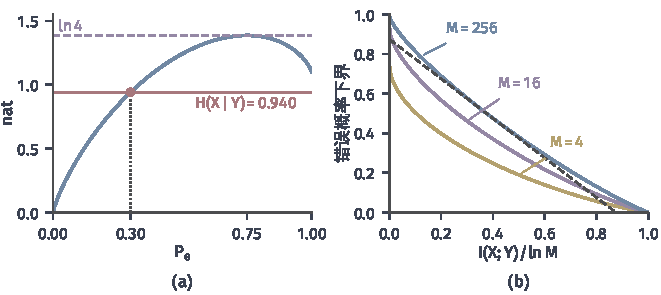
\includegraphics[width=112mm]{figures/07-probability/04-distribution-analysis/matplotlib/info-fano/figure.pdf}
  \caption{Fano不等式。(a)$M=4$时$\phi_4(P_{\mathrm{e}})=h_{\mathrm{b}}(P_{\mathrm{e}})+P_{\mathrm{e}}\ln3$（蓝），在$P_{\mathrm{e}}=\tfrac34$处达到$\ln4$（紫虚线）。红线为四值对称观测例子的$H(X\mid Y)\approx0.940$，与曲线交于$P_{\mathrm{e}}=0.3$。(b)$X$均匀时Fano给出的最小错误概率，横轴为$I(X;Y)/\ln M$，$M=4,16,256$；灰虚线为$M=256$时式~\eqref{eq:info-fano-mi}的较弱形式。}
  \label{fig:info-fano}
\end{BookInlineFigure}

等号成立的条件从证明中可以读出：每个$y$下错误概率相同（Jensen取等），并且猜错时其余$M-1$个值等可能。上面的例子两条都满足。一般情形下Fano不等式只是下界，实际最小错误可以大得多。

定理只适用于有限个标签和“猜错与否”这种错误标准。若要估计的是连续参数，“猜中”的概率通常为零，不等式不能直接使用；需要先从参数中挑出有限个相互分开的候选，把估计问题改写成在它们之间辨别，下一小节会看到这种改写的样子。

\subsection{通信与统计辨别}
\label{sec:info-fano-applications}

当$X$在$M$个标签上均匀时，$H(X)=\ln M$，由式~\eqref{eq:info-mi-entropy-difference}，$H(X\mid Y)=\ln M-I(X;Y)$。这里$Y$可以不是离散的，第~\ref{sec:info-mi-entropy}节的证明逐个条件值进行，同样成立。代入较弱形式（这次用$\ln M$代替$\ln(M-1)$，对$M=2$也适用），得到
\begin{equation}
  P_{\mathrm{e}}\geq1-\frac{I(X;Y)+\ln2}{\ln M}.
  \label{eq:info-fano-mi}
\end{equation}
这个形式只需要互信息：要以小错误区分$M$个等可能的标签，观测至少要提供约$\ln M$的信息。四值对称观测的例子中$I(X;Y)=\ln4-0.940\approx0.446$，式~\eqref{eq:info-fano-mi}给出$P_{\mathrm{e}}\geq0.178$，比精确形式的$0.3$弱。图~\ref{fig:info-fano}(b)比较了不同$M$时的精确下界：横轴按$\ln M$归一化后，$M$越大，曲线越接近直线$1-I/\ln M$。

\paragraph{通信}
在有噪声的线路上传送消息时，消息$W$从$M$个中均匀选出，编码成线路输入$X_1,\dots,X_n$，线路输出$Y_1,\dots,Y_n$，接收方据此猜出$\hat{W}$。码率$R=\ln M/n$是每次使用线路平均传送的信息。由于$\hat{W}$只依赖输出，$W\to(Y_1,\dots,Y_n)\to\hat{W}$；由于输出只经由输入依赖消息，数据处理不等式给出
\[
  I(W;Y_1,\dots,Y_n)\leq I(X_1,\dots,X_n;Y_1,\dots,Y_n).
\]
第~\ref{chap:discrete-channel-capacity}章会证明，对每次使用相互独立的线路，右端不超过$nC$，$C$是单次使用的容量。代入式~\eqref{eq:info-fano-mi}，得到
\[
  P_{\mathrm{e}}\geq1-\frac{nC+\ln2}{nR}=1-\frac{C}{R}-\frac{\ln2}{nR}.
\]
若$R>C$，$n\to\infty$时右端趋于$1-C/R>0$，错误概率不能趋于零。这里的错误概率是按均匀消息平均的；逐个消息的最大错误概率不小于平均值，下界对它同样成立。

\paragraph{统计辨别}
设有$M$个候选分布$P_1,\dots,P_M$，标签$J$均匀选出，观测是来自$P_J$的独立同分布样本$X_1,\dots,X_n$，要从样本猜出$J$。这时需要的是$I(J;X_1,\dots,X_n)$的上界。

离散情形下，对任意分布$Q$，记$\bar{P}=\tfrac1M\sum_jP_j$为观测的边缘分布，在各项有限时直接展开对数可以核对
\[
  \frac1M\sum_{j=1}^{M}D_{\mathrm{KL}}(P_j\Vert Q)=I(J;X)+D_{\mathrm{KL}}(\bar{P}\Vert Q),
\]
依据是对数比的拆分
\[
  \ln\frac{p_j(x)}{q(x)}=\ln\frac{p_j(x)}{\bar{p}(x)}+\ln\frac{\bar{p}(x)}{q(x)}.
\]
按权重$\tfrac1Mp_j(x)$对$j$与$x$求和，第一项给出$I(J;X)$（$(J,X)$的联合质量是$\tfrac1Mp_j(x)$，边缘乘积是$\tfrac1M\bar{p}(x)$），第二项给出$D_{\mathrm{KL}}(\bar{P}\Vert Q)$。右端第二项非负，所以
\[
  I(J;X)\leq\frac1M\sum_{j=1}^{M}D_{\mathrm{KL}}(P_j\Vert Q).
\]
取$Q$为某个候选$P_k$，就得到$I(J;X)\leq\max_{j,k}D_{\mathrm{KL}}(P_j\Vert P_k)$。$n$个独立样本时，乘积分布的对数比是各样本对数比之和，KL随之乘以$n$。于是
\[
  P_{\mathrm{e}}\geq1-\frac{n\max_{j,k}D_{\mathrm{KL}}(P_j\Vert P_k)+\ln2}{\ln M}.
\]

例如$M=8$个候选$\mathcal{N}(\theta_j,1)$，$\theta_j=0,0.1,\dots,0.7$。按定义计算，
\[
  D_{\mathrm{KL}}\bigl(\mathcal{N}(a,1)\Vert\mathcal{N}(b,1)\bigr)=\mathbb{E}\Bigl[\frac{(X-b)^{2}-(X-a)^{2}}{2}\Bigr]=\frac{(a-b)^{2}}{2},
\]
期望对$X\sim\mathcal{N}(a,1)$取。最大值是$0.7^{2}/2=0.245$，一个样本时$P_{\mathrm{e}}\geq1-(0.245+\ln2)/\ln8\approx0.549$。候选越密、样本越少，辨别越难；要让下界失效，样本数须与$\ln M/\max D_{\mathrm{KL}}$同阶。

这两个应用用的是同一个工具，但要分别核对三件事：标签是否均匀（Fano给的是平均错误）、观测是怎样由标签产生的（决定互信息的上界）、错误按什么标准计算。把估计连续参数的误差转成在候选之间的辨别错误，是卷八的工作，可参考\BookChapterRef{chap:finite-sample-lower-bounds}{卷八第5章“有限样本的精度下界”}。
